\documentclass{standalone}
\usepackage{tikz}
\usepackage{amsmath}
\usepackage{fontspec}
\usetikzlibrary{patterns}

%: === TIPOGRAFÍA === (((
\setmainfont[
  BoldFont       = bodonibi,
	ItalicFont     = Century modern italic2.ttf,
	BoldItalicFont = bodonibi,
	SmallCapsFont  = lmromancaps10-regular.otf
]{Century_modern.ttf}
\DeclareSymbolFont{italics}{\encodingdefault}{\rmdefault}{m}{it}
\DeclareSymbolFontAlphabet{\mathit}{italics}
\ExplSyntaxOn
\int_step_inline:nnnn { `A } { 1 } { `Z }
 {  \exp_args:Nf \DeclareMathSymbol{\char_generate:nn{#1}{11}}{\mathalpha}{italics}{#1} }
\int_step_inline:nnnn { `a } { 1 } { `z } {  \exp_args:Nf \DeclareMathSymbol{\char_generate:nn{#1}{11}}{\mathalpha}{italics}{#1}}
\ExplSyntaxOff
% )))

\begin{document}

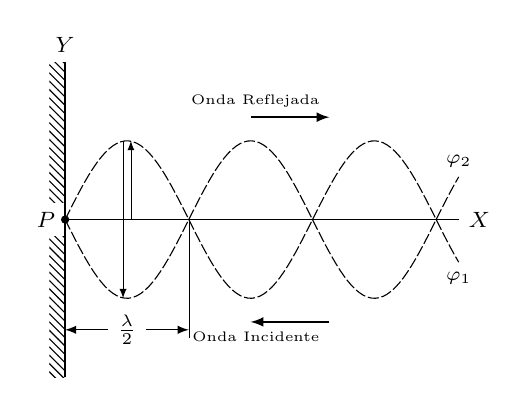
\begin{tikzpicture}[>=latex]
	\fill [pattern = north west lines] (0,-2) rectangle (-0.2,2);
	\draw [semithick] (0,-2) -- (0,2) node [above] {\footnotesize \(Y\)} (0,0) node [left, fill=white] {\footnotesize \(P\)} -- (5,0) node [right] {\footnotesize \(X\)};
	\draw [dash pattern = on 4pt off 1pt, domain=0:5, samples = 100] plot(\x , {sin(2*\x r)}) node [below] {\scriptsize \(\varphi _1\)};
	\draw [dash pattern = on 4pt off 1pt, domain=0:5, samples = 100] plot(\x , {-sin(2*\x r)}) node [above] {\scriptsize \(\varphi _2\)};
	\draw [very thin] (pi/2,0) --++ (0,-1.5);
	\draw [<->] (0,-1.4) to node[midway,fill=white] {\footnotesize \(\frac{\lambda}{2}\)} ++ (pi/2,0);
	\draw [semithick,->] (3*pi/4,1.3) --++ (1,0) node [above left] {\tiny Onda Reflejada};
	\draw [semithick,<-] (3*pi/4,-1.3) --++ (1,0) node [below left] {\tiny Onda Incidente};
	\draw [very thin, ->] (pi/4+0.05,0) --++ (0,1);
	\draw [very thin, ->] (pi/4-0.05,1) --++ (0,-2);
	\fill (0,0) circle (1.5pt);
\end{tikzpicture}

\end{document}
